%!TEX root = ../my_thesis.tex
\chapter{Techniques for fast z feedback}

Several people have improved the AFM feedback loop by implementing model based controller or high frequency actuators. The drawback with these actuators is the decrease in the positioning range.
/CURRENT FEEDBACK SCHEME

We have decided to improve the bandwidth and the scan range of our device. 
Many people have improved the bandwidth of their AFM by designing a dual integrated actuators system \cite{sulchek1999dual}. Most of them have introduced an external piezoelectrical actuator on top of the cantilever. With this scheme, we can combine the advantages of a high bandwidth from the piezo-electrical actuator and the long range of the tip.

/PREVIOUS METHOD OF TILT

\section{Double PID}

The principal feature of an AFM is it's probing system. \cite{jeong:093706} The feedback control system is designed to adjust the motion of the tip on the z-axis. It will adjust the tip-to-sample distance. We have developed a dual-actuator control system. 

We put a piezo-electrical ceramics on top of the X-Y scanner. This device will work with the scanner to achieve a larger bandwidth. Indeed, it picks up high spatial frequency topography. 

\begin{figure}[H]
  \centering
  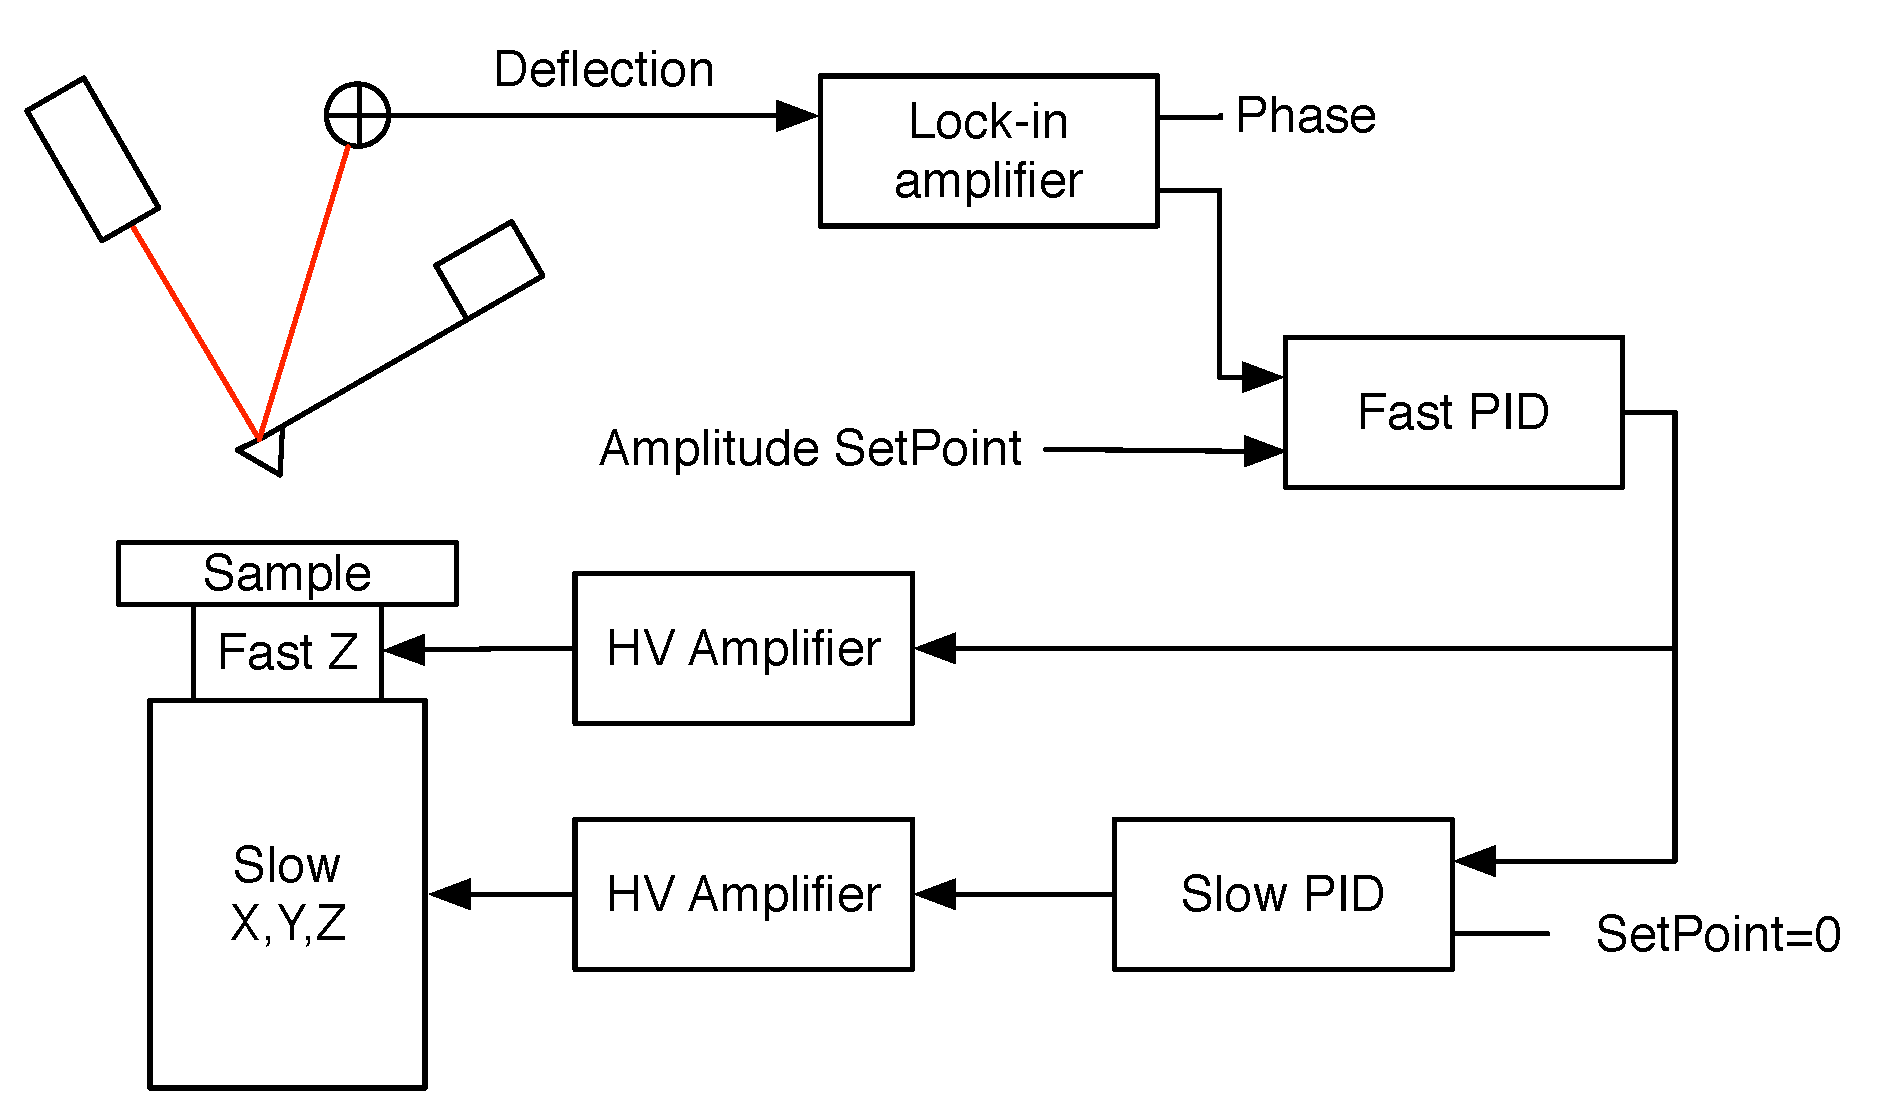
\includegraphics[scale=0.3]{images/doublePID.eps}
    \caption{Double PID}
  \label{DoublePid}
\end{figure}

\section{Tilt compensation}

In theory, the mounted sample should be flat: parallel to the XY-Scanner. If the probe/sample angle is not perpendicular, we observe a tilt on the surface. This tilt is problematic when it becomes larger than the features. There are multiple ways to compensate for this. The most common technique is to use post processing to adjust the acquired data. Flattening algorithms or first-order planefitting restore the image and put the data on the same level. This technique works if the range of the tip is large enough. We have decided to take another approach and to dynamically compensate for the tilt. Before performing our scan, we will do a first scan to compute the tilt of the sample by considering our tilt as a 3D plane. Then, we'll generate a tilt correction signal that will be added to z scan output.

We use a circle pattern to scan the surface of the sample. The radius of the circle is equal to the scan size. It gives us informations about the general topography of the surface. Then, we compute the plane equation of the surface by applying a fit in Igor Pro. This fit will generate a plane that models the tilted surface. The input of this fit are the theoretical X-Y output waves of the circle pattern: a sinus and a cosines. The data on the z axis is the height.

\begin{equation}\label{eqn:planeeq}
z = a_1 x + a_2 y + a_3 
\end{equation}

The coefficients by minimizing the values of Chi-Square (error function). Then, we generate the waves to send to the controller the following way.

\begin{equation}\label{eqn:sendwave}
wavetosend = a_1 wavex + a_2 wavey 
\end{equation}

Wavex and wavey are the output of our scan pattern. With this method, we can do a tilt correction with any scan pattern.


\subsection{Experiment}

Wavex and wavey are the x,y components of our scan pattern. The scan pattern for an Archimedean spiral is defined by the equation  ~\ref{eqarchimedean}.

\begin{equation}\label{eqarchimedean}
x(t)= \alpha \sqrt{t} cos(\beta \sqrt{t})\\
y(t)= \alpha \sqrt{t} sin(\beta \sqrt{t})
\end{equation}

We took a calibration sample to test the efficiency of our method. The size or our scan is 30um. We see on the figure  ~\ref{tiltcircle} that the surface has a tilt. The small spikes on the curve represent the pyramids on the sample.


\begin{figure}[H]
  \centering
  \includegraphics[scale=0.3]{images/tiltcircles.eps}
    \caption{Output of the tilt pattern}
  \label{tiltcircle}
\end{figure}

Then we compute our fitting algorithm on the x,y and z data.
\begin{table}[H]
\caption{Planefit coefficients} % title of Table
\centering % used for centering table
\begin{tabular}{c c c} % centered columns (4 columns)
\hline\hline %inserts double horizontal lines
$a_1$ & $a_2$ & $a_3$ \\ [0.5ex] % inserts table 
%heading
\hline % inserts single horizontal line
-0.14615  & -0.031882 & 29.537 \\[1ex]

\hline %inserts single line
\end{tabular}
\label{table:planefit} % is used to refer this table in the text
\end{table}

The size of the scan is still 30 $\mu m$ and the spiral has 80 loops. The scan pattern we are going to send to the controller is generated with the previously computed planefit coefficients. 

\begin{figure}[H]
  \centering
  \includegraphics[scale=0.1]{images/spiralztiltout.eps}
    \caption{Input of the tilt compensation}
  \label{spiralztiltout}
\end{figure}



\begin{figure}[H]
  \centering
  \includegraphics[scale=0.1]{images/tiltcorrectiongraph.eps}
    \caption{Output of the fast piezo}
  \label{spiralzfast}
\end{figure}


The tilt compensation will take a load off the small fast piezoelectrical ceramics. The Figure ~\ref{spiralzfast} shows the efficiency of our method. Indeed, the fast piezo was previously saturating. The piezos was trying to reach features that are larger than his range. If we use the tilt correction, we see that our piezo has no problem reaching those features.
